\section{The Gamma function}

\subsection{Definition}

The \textit{gamma function} was introduced by Leonhard Euler in his goal to generalize the factorial to non-integer values.

\begin{definition}[Euler, 1970]
    Let $x > 0$. We define:
    \[
        \Gamma(x) = \int_0^1 (-\log t)^{x - 1} \, dt
    \]   
\end{definition}

\begin{theorem}
    For $x > 0$,
    \[
        \Gamma(x) = \int_0^\infty t^{x - 1} e^{-t} \, dt
    \]
\end{theorem}
\begin{proof}
    Use the change of variable $u = -\log t, \ t = e^{-u}, \ dt = -e^{-u} du$. Note that $t \rightarrow 0 \implies u \rightarrow \infty$, and $t \rightarrow 1 \implies u \rightarrow 0$.
\end{proof}

The derivatives can be deduced by differentiating under the integral sign of the second expression:
\[
    \Gamma'(x) = \int_0^\infty t^{x - 1} e^{-t} \log(t) \, dt
\]
\[
    \Gamma^{(n)}(x) = \int_0^\infty t^{x - 1} e^{-t} \log^n(t) \, dt
\]

\begin{remark}
    Remember that $t = e^{\log(t)}$, and then: $t^{x - 1} = (e^{\log(t)})^{x - 1} = e^{\log(t) (x - 1)}$. Thus, $\frac{d}{dx} t^{x - 1} = \log(t) e^{\log(t) (x - 1)} = \log(t) t^{x - 1} $
\end{remark}

\subsection{Properties}

\subsubsection{The functional equation}

We have that
\[
    \Gamma(1) = \int_0^\infty e^{-t} \, dt = 1
\]
and, for $x > 0$, an integration by parts ($u = t^{x - 1}, \frac{du}{dt} = t^{x - 2}, v = e^{-t}, \frac{dv}{dt} = -e^{-t}$) yields:
\[
    \Gamma(x + 1) = \int_0^\infty t^x e^{-t} \, dt = [-t^x e^{-t}]_0^\infty + x \int t{x - 1} e^{-t} \, dt = x\Gamma(x)
\]
and the relation $\Gamma(x + 1) = x \Gamma(x)$ is the important \textbf{functional equation}.

For integers the functional equation becomes:
\[
    \Gamma(n + 1) = n!
\]
and it’s why the gamma function can be seen as an extension of the factorial function to real non null positive numbers.

\subsubsection{Other important values}

\[
    \Gamma\left(\frac{1}{2}\right) = \int_0^\infty \frac{e^{-t}}{\sqrt{t}} \, dt = 2\int_0^\infty e^{-u^2} \, du = 2 \frac{\sqrt{\pi}}{2} = \sqrt{\pi}
\]

\subsubsection{Plot}

\begin{figure}[H]
    \centering
	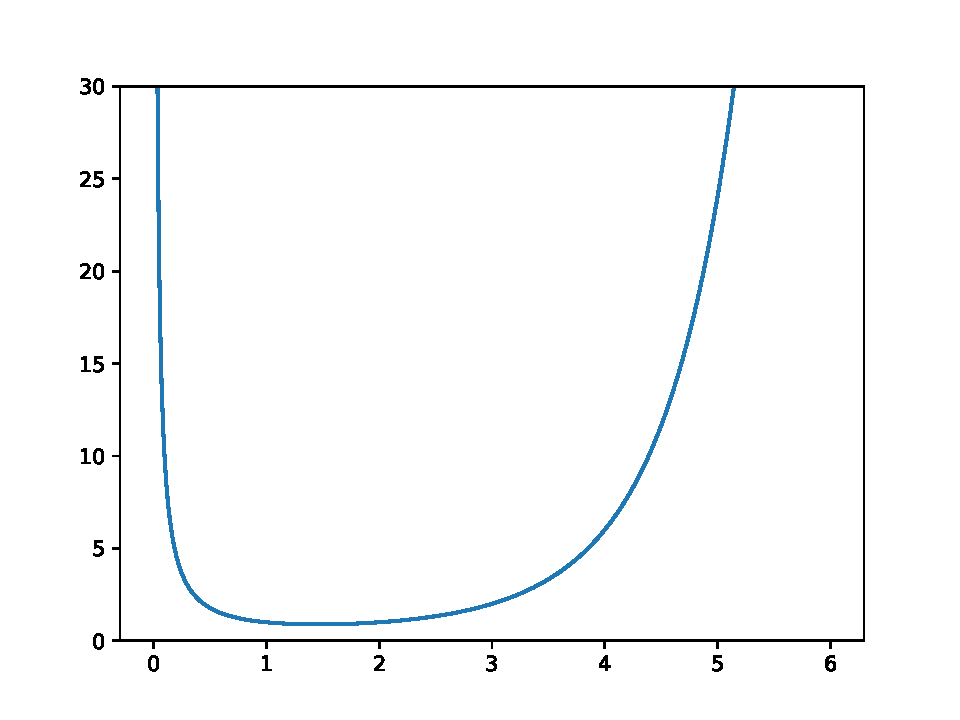
\includegraphics[width=0.5\textwidth]{appendices/gamma.pdf}
\end{figure}

\section{The beta function}

\subsection{Definition}

We define the \textit{beta function} as

\[
    \beta(x, y) = \int_0^1 t^{x - 1}(1 - t)^{y - 1} \, dt
\]

\subsection{Properties}

\begin{prop}
The beta function is symmetric:
\[
    \beta(x, y) = \beta(y, x)
\]
\end{prop}
\begin{proof}
    Because of the convergent property of definite integrals,
    \[
        \int_0^a f(t) \, dt = \int_0^a f(a - t) \, dt
    \]  
    we can rewrite the above integral as
    \[
        \beta(x, y) = \int_0^1 (1 - t)^{x - 1} t^{y - 1} \, dt = \int_0^1 t^{y - 1} (1 - t)^{x - 1} \, dt = \beta(y, x)
    \]
\end{proof}

\begin{prop}
    The following relation between the gamma and beta functions holds:
    \[
        \beta(x, y) = \frac{\Gamma(x) \Gamma(y)}{\Gamma(x + y)}
    \]
    Then, for positive integers $x$ and $y$ we can define the beta function as:
    \[
        \beta(x, y) = \frac{(x - 1)! (y - 1)!}{(x + y - 1)!}
    \]
\end{prop}
\begin{proof}
    Using the definition of the gamma function, we can write
    \[
        \Gamma(m)\Gamma(n) = \int_0^\infty x^{m - 1} e^{-x} \, dx \int_0^\infty y^{n - 1} e^{-y} \, dy
    \]
    Then we can rewrite it as a double integral
    \[
        \Gamma(m)\Gamma(n) = \int_0^\infty \int_0^\infty x^{m - 1} y^{n - 1} e^{-(x + y)} \, dx dy
    \]
    Applying the substitution $x = vt$ and $y = v(1 - t)$, we have
    ...
\end{proof}

https://brilliant.org/wiki/beta-function/